%! TEX program = lualatex
\documentclass[12pt,a4paper]{article} 

% Packages for formatting
\usepackage{fontspec}
\usepackage[ngerman]{babel}
\usepackage{geometry} 
\geometry{margin=1in} 
\usepackage{setspace} 
\usepackage{hyperref} 
\usepackage{xcolor}
\usepackage{amsmath} % for align*
\usepackage{amsthm} % neue Theorem-Umgebungen
\usepackage{enumitem} % für schöne Listen (Teilaufgaben)
\usepackage{mathbbol}
\usepackage{graphicx}
\usepackage{amssymb}
\usepackage{gensymb}

% Style settings
%\pagecolor{darkgray}      % sets background color to black 
%\color{gray}          % sets text color to white

% Change subsection to use a, b, c instead of 1, 2, 3
\renewcommand{\thesubsection}{\alph{subsection})}

% Title page info 
\title{Blatt 07}
\author{Hannes Rall \\ Albert-Ludwigs-University}
\date{\today}

\begin{document}
% Title page 
\begin{titlepage}
    \centering
    \vspace*{2cm}
    {\Huge\itshape Blatt 07\par}
    \vspace{2cm}
    {\Large\textsc{Hannes Rall}\par}
    \vfill
    {\large Albert-Ludwigs-University\\}
    \vspace{1cm}
    {\large\today\par}
\end{titlepage}
\newpage
\section*{Aufgabe 19}
Schon in der Grundschule werden Parkettierungen genutzt, um das Erkennen
von Mustern und Strukturen zu fördern (Parkette legen, Parkette weiterzeichnen, Parkette selbst erfinden, . . . ).
Solche Parkette stellt man sich so vor, dass sie sich unendlich in der Ebene fortsetzen. Die Regelmäßigkeiten, die
solchen Mustern zu Grunde liegen, lassen sich mathematisch mit Hilfe von Kongruenzabbildungen/Symmetrien
beschreiben. Diese bilden mit der Hintereinanderausführung immer eine Gruppe, die Symmetriegruppe des
jeweiligen Musters. Diese ist immer eine Untergruppe aller Kongruenzabbildungen der euklidischen Ebene.
\subsection*{(ia)}
Jede Symmetrie eines Musters in der Ebene ist eine Verschiebung, Drehung, Rotation oder eine Gleitspiegelung. Ist das Muster nur endlich ausgedehnt kann es nur eine Rotation oder eine Spiegelung sein.\\

\begin{figure}[htbp]
    \centering
    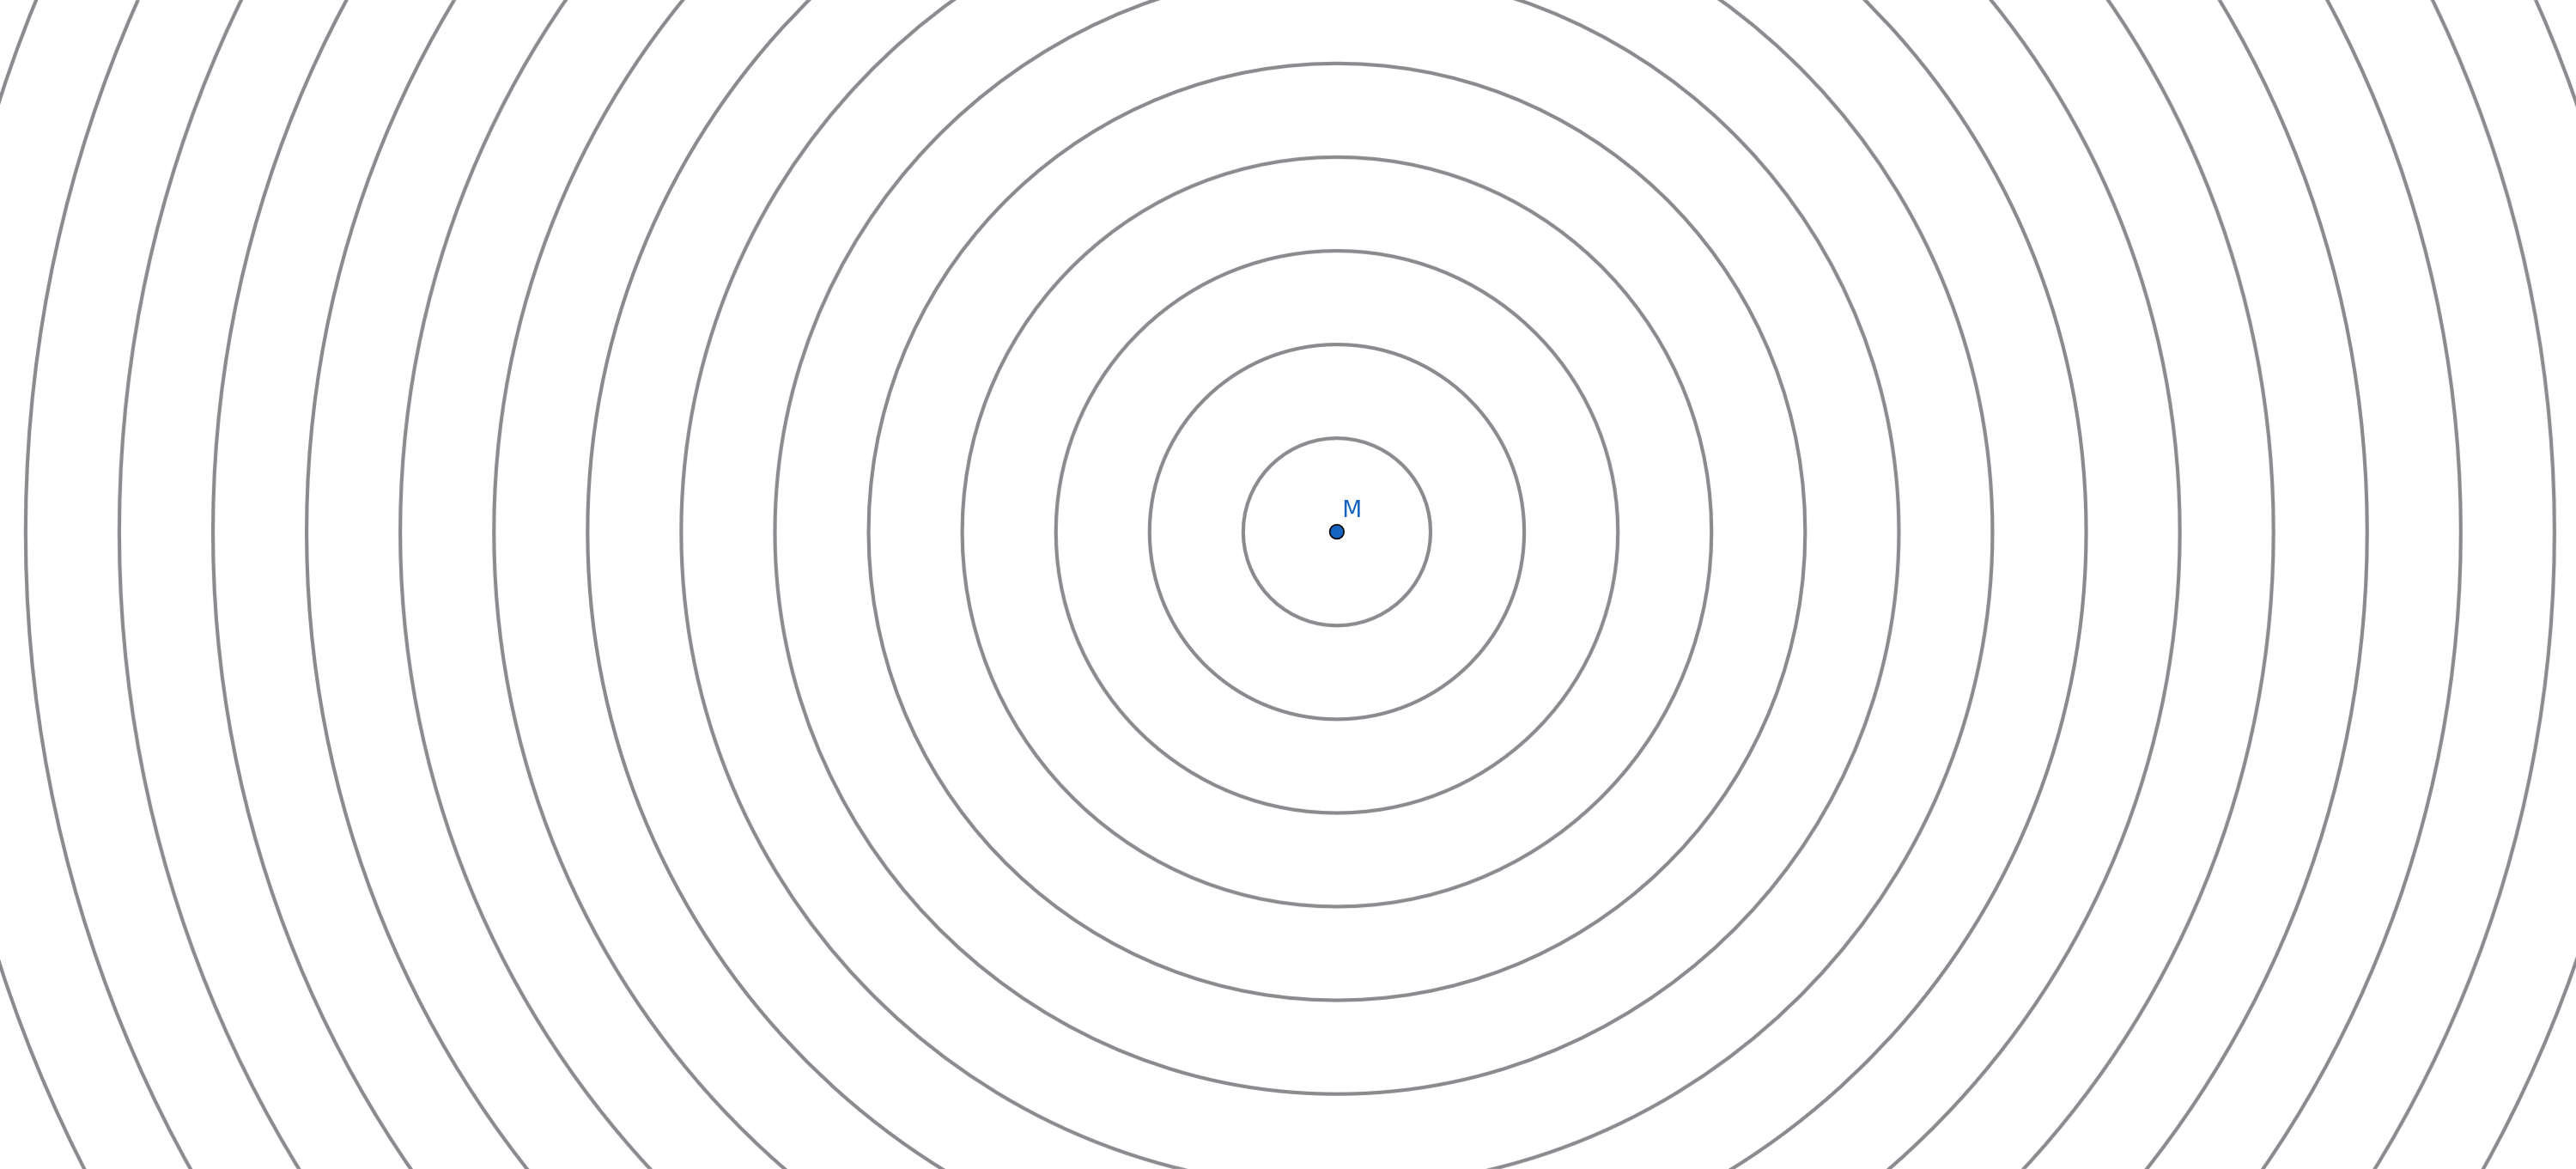
\includegraphics[width=0.8\textwidth]{Blatt07_Aufgabe_19_ia.png}
    \caption{Muster}
    \label{fig:Aufgabe_19}
\end{figure}

\noindent Ein Muster, dessen Symmetriegruppe nicht endlich erzeugt ist, wären Kreise um Kreise. Also man nimmt sich einen Punkt M und für alle $r \in \mathbb{N}$ zeichnet man einen Kreis $K_r$ mit dem Radius r mit Mittelpunkt M. Für alle möglichen Winkel ist die Rotation um M in der Symmetriegruppe enthalten und für jede Gerade die durch den Mittelpunk M geht ist die Spiegelung an der Geraden auch in der Symmetriegruppe enthalte. Da es überabzählbar viele solche Rotationen und Spiegelungen gibt, muss die Symmetriegruppe unendlich erzeugt sein.\\

\newpage
\subsection*{(ib)}
\noindent Hier sollte man zunächst alle Verschiebungen finden. Diese bilden eine Untergruppe aller Symmetrien des Musters. Die Größe eines minimalen Erzeugendensystems aller Verschiebungen ist (falls die
Verschiebungen endlich erzeugt und nicht nur aus der Identität bestehen) 1 oder 2.\\
Muster bei dem das Erzeugendensystems aller Verschiebungen die Größe 1 hat:
\begin{figure}[htbp]
    \centering
    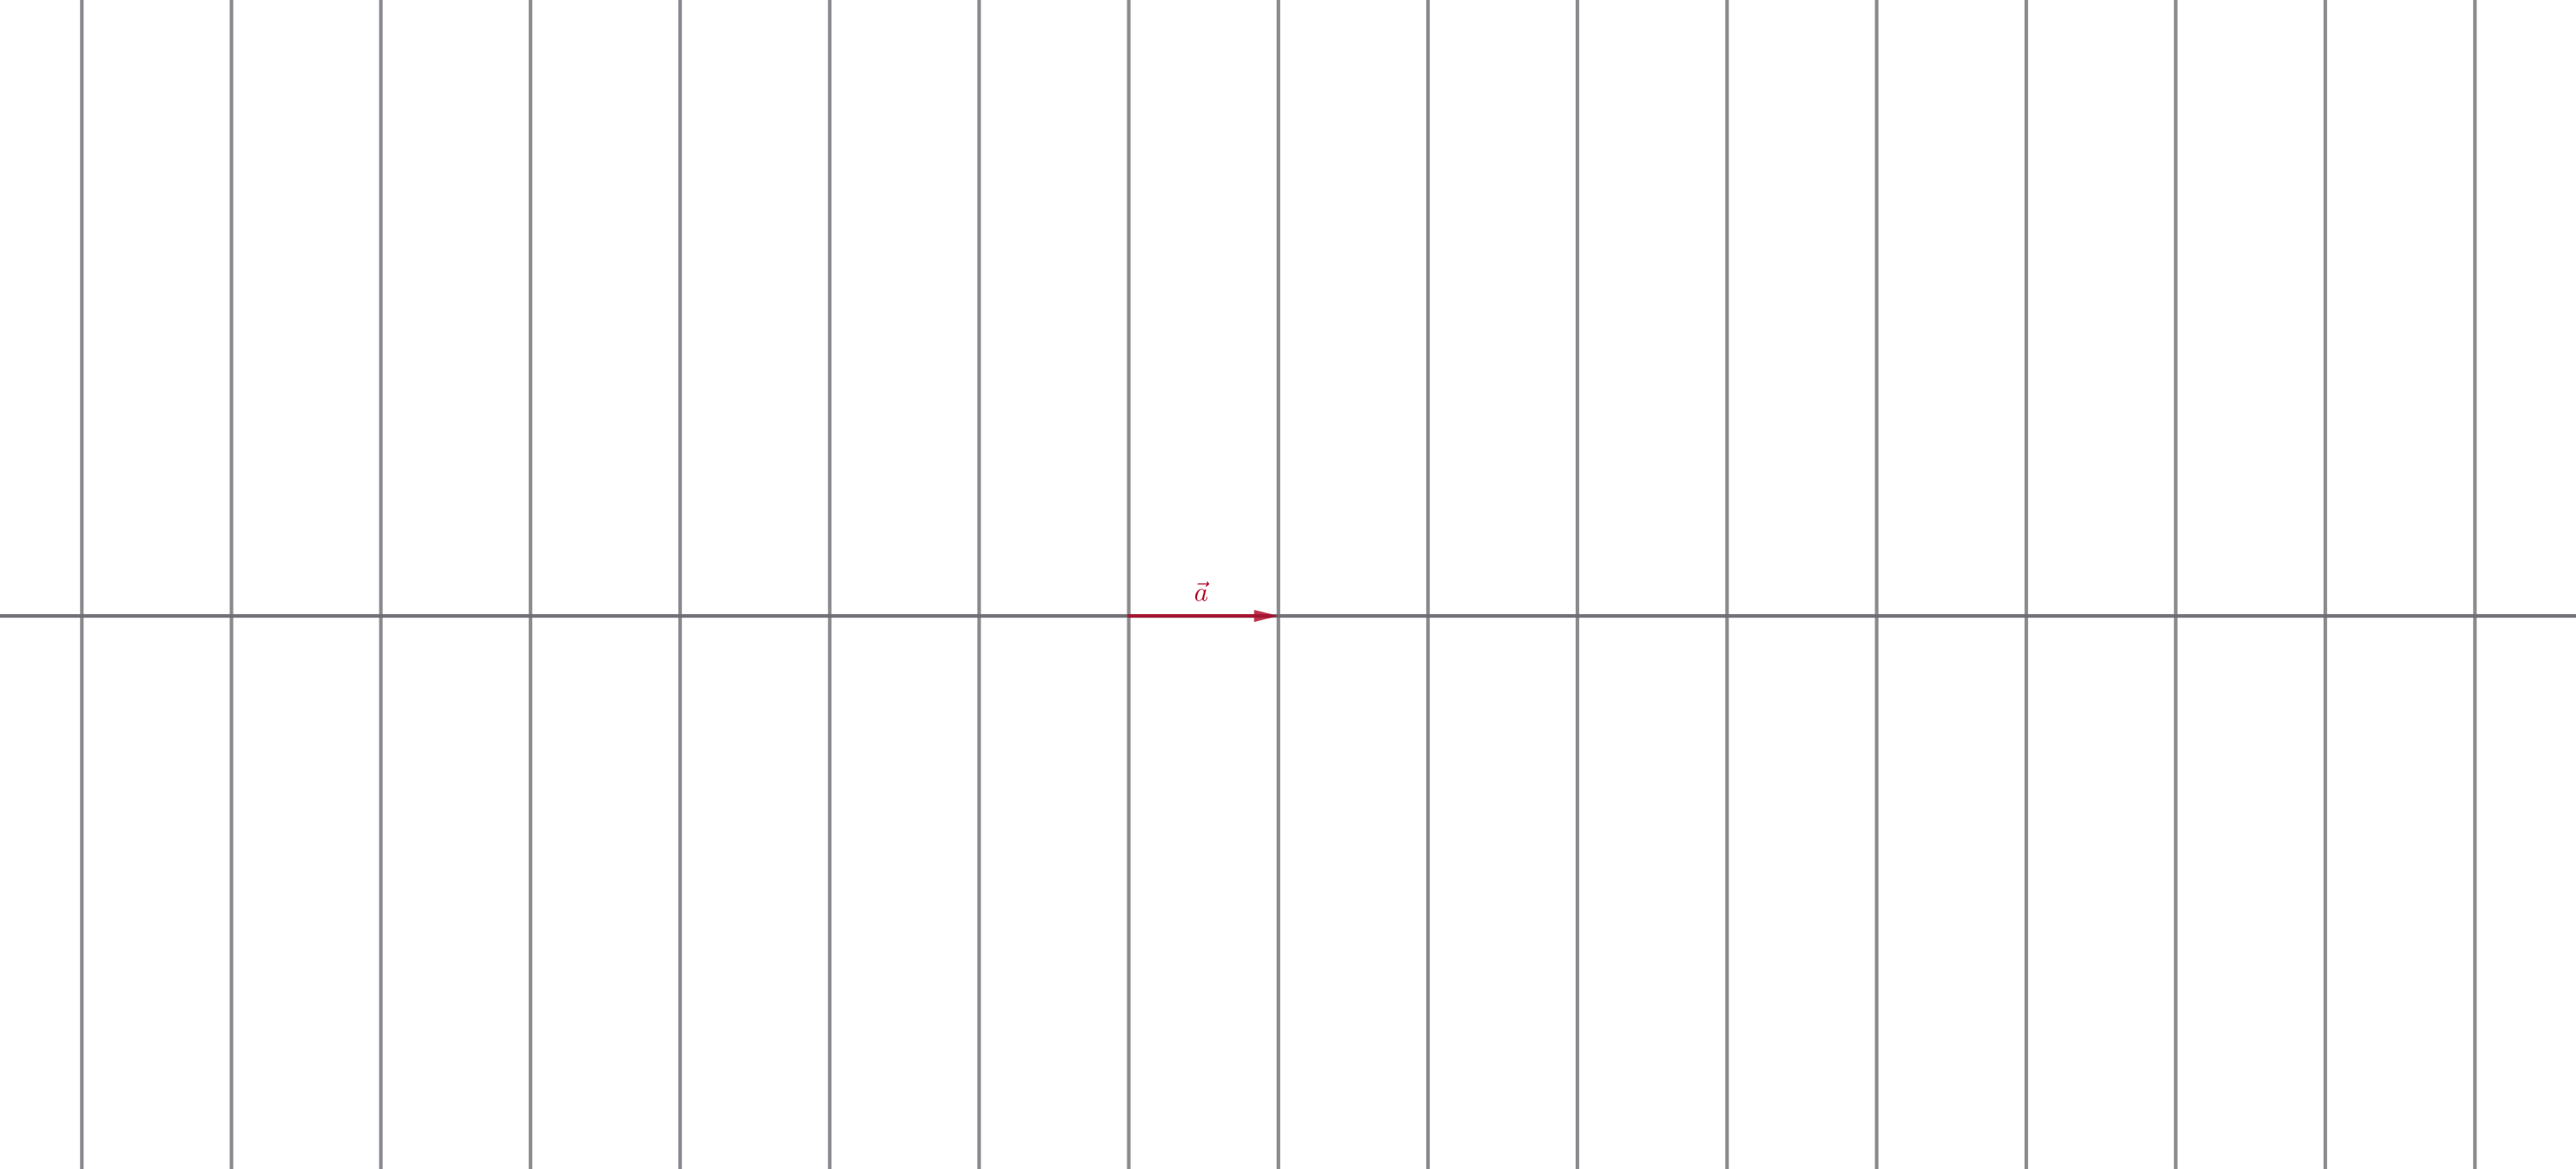
\includegraphics[width=0.8\textwidth]{Blatt07_Aufgabe_19_ib_1.png}
    \caption{Muster}
    \label{fig:Aufgabe_19}
\end{figure}
\\
Bei diesem Muster ist nur eine Verschiebung entlang der horizontalen Geraden möglich, und zwar jeweils um ein Vielfaches des eingezeichneten Vektors $\vec{a}$. Andere Verschiebungen sind aufgrund der horizontalen Geraden nicht möglich. Das Erzeugendensystems besteht also aus der Verschiebung um den Vektor $\vec{a}$.\\
\\
Muster bei dem das Erzeugendensystems aller Verschiebungen die Größe 2 hat:
\begin{figure}[htbp]
    \centering
    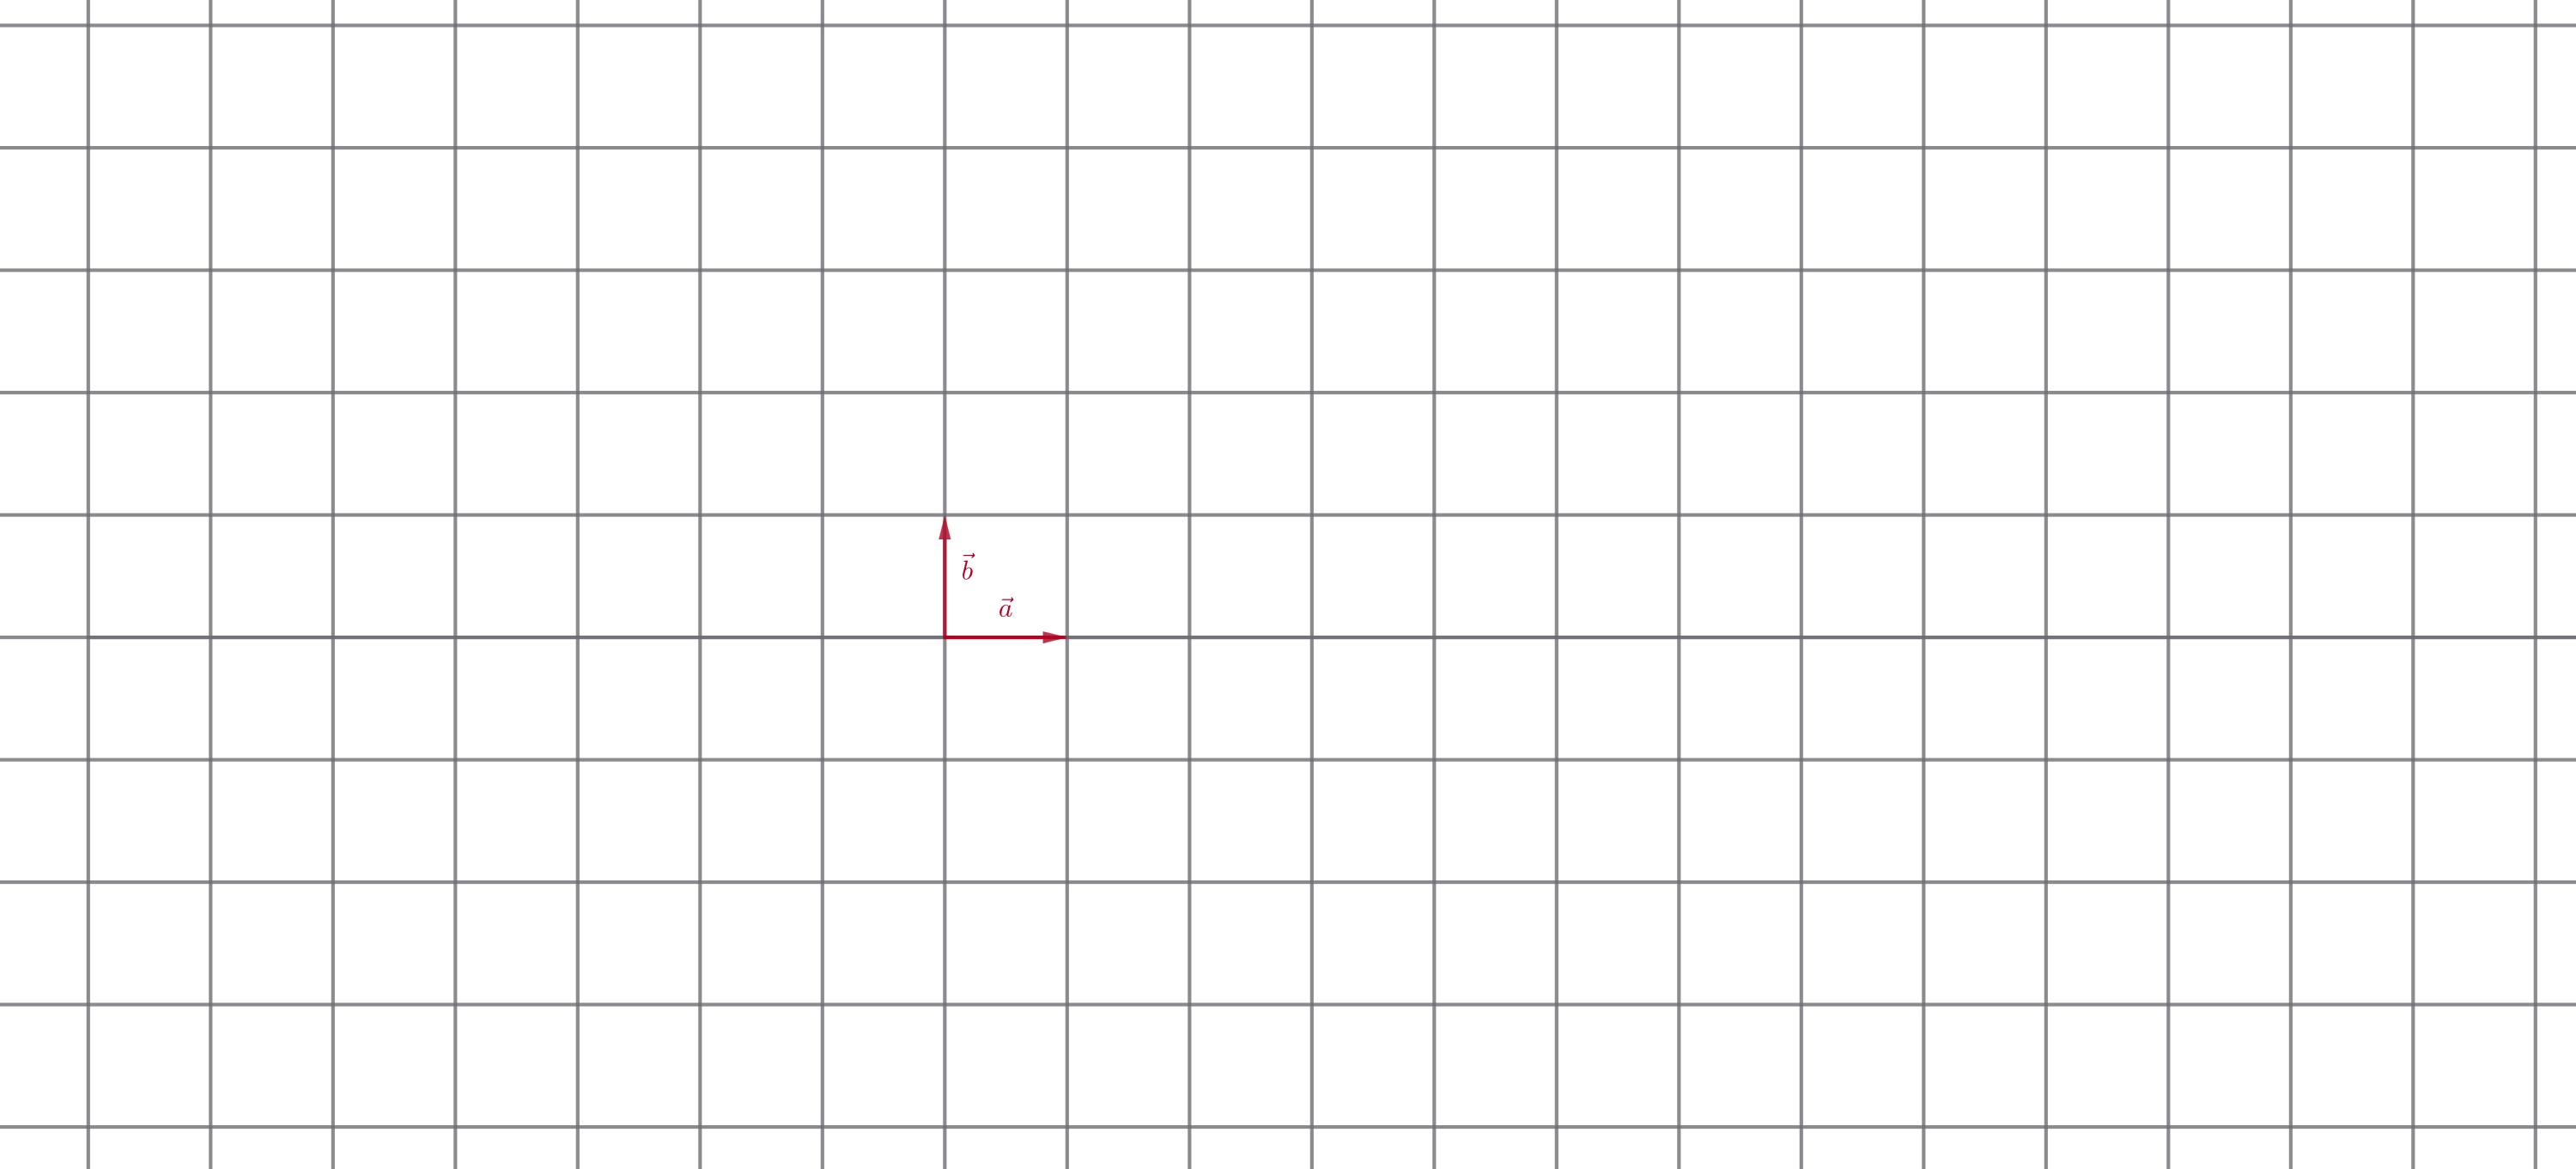
\includegraphics[width=0.8\textwidth]{Blatt07_Aufgabe_19_ib_2.png}
    \caption{Muster}
    \label{fig:Aufgabe_19}
\end{figure}
\\
Bei diesem Muster ist eine Verschiebungen sowohl entlang der horizontalen als auch der vertikalen Geraden möglich. Das Erzeugendensystems besteht also aus den Verschiebungen um die eingezeichneten Vektoren $\vec{a}$ und $\vec{b}$.\\
Zeichnet man die zugehörigen Verschiebungsvektoren (beginnend bei einem beliebigen aber für alle Vektoren festen Punkt) ins Muster ein, so spannen diese Vektoren im ersten Fall einfach nur den Vektor selbst und im zweiten Fall ein Parallelogramm auf – in beiden Fällen nennt man dies eine Translationszelle.

\subsection*{(ic)}
\noindent Als nächstes finden wir alle Spiegelungen. Dabei hilft: Für eine Spiegelung sg, die Symmetrie des Musters ist, gibt es auch eine Spiegelung sh, die Symmetrie des Musters ist, so dass h einen Anteil (ein Intervall) hat, der in oder auf dem Rand der Translationszelle verläuft.\\
\\
Begründung:\\
Jede Spiegelung, die das Muster invariant lässt, muss mit den Verschiebungen verträglich sein. Da das Muster periodisch ist, gibt es zu jeder Spiegelachse g äquivalente Spiegelachsen durch Verschiebung. Man kann daher immer eine Spiegelachse h finden, die durch die Translationszelle (oder ihren Rand) verläuft, indem man g geeignet verschiebt (modulo der Translationszelle). Damit ist h eine zu g äquivalente Spiegelachse innerhalb der Zelle.

\subsection*{(id)}
Als nächstes finden wir alle Drehungen.\\
Für jede Drehung, die Symmetrie des Musters ist, gibt es auch eine Drehung mit einem Drehzentrum, das in oder auf dem Rand der Translationszelle liegt.\\
\\
Begründung:\\
Da das Muster periodisch ist, gibt es zu jedem Drehzentrum äquivalente Drehzentren durch Verschiebung. Man kann daher immer ein Drehzentrum innerhalb oder auf dem Rand der Translationszelle finden, indem man das ursprüngliche Zentrum geeignet verschiebt (modulo der Translationszelle).

\subsection*{(ie)}
Nun bleiben noch die Gleitspiegelungen. Es kann Gleitspiegelgungen geben, wo die Verschiebung und Spiegelung aus der sie zusammengesetzt sind, nicht sowieso schon selbst Symmetrien des Musters sind.\\
Beispiele hierfür sind spezielle Friesgruppen (Bandornamente):\\
\begin{figure}[htbp]
    \centering
    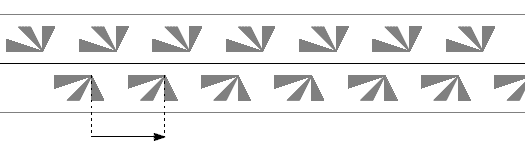
\includegraphics[width=0.8\textwidth]{Blatt07_Aufgabe_19_ie.png}
    \caption{Muster}
    \label{fig:Aufgabe_19}
\end{figure}
\\
Es gibt keine Spiegelungen, da nur die mittlere horizontalen Gerade g, paralelle Geraden zu g oder senkrechte Geraden zu g in Frage kämen. Jedoch sind die Figuren nicht vertikal symmetrisch und so verschoben, dass auch g und paralelle Geraden zu g nicht in Frage kommen.\\
\\
\noindent Wir suchen nun nur Gleitspiegelungen, wo die Verschiebung und Spiegelung aus der sie zusammengesetzt sind, nicht sowieso schon selbst Symmetrien des Musters sind. Denn die anderen werden schon durch die zuvor gefundenen Symmetrien erzeugt.\\
\\
Die Hintereinanderausführung einer Gleitspiegelung1 $v_{\vec{a}} \circ s_g $mit sich selbst ist immer eine Verschiebung
$v_{2\vec{c}}$ , wobei $\vec{c}$ der zu g parallele Anteil von $\vec{a}$ ist (d.h. $\vec{a} - \vec{c}$ ist senkrecht zu g).\\
Sei $s_g$ die Spiegelung an der Geraden $g$ und $v_{\vec{a}}$ die Verschiebung um $\vec{a}$.\\
\\
Die Hintereinanderausführung ist:
\[
(v_{\vec{a}} \circ s_g) \circ (v_{\vec{a}} \circ s_g) = v_{\vec{a}} \circ s_g \circ v_{\vec{a}} \circ s_g
\]
\\
Da 
\[
s_g \circ v_{\vec{a}} = v_{s_g(\vec{a})} \circ s_g
\]
(gilt, weil die Spiegelung die Verschiebung um $\vec{a}$ in eine Verschiebung um $s_g(\vec{a})$ überführt), ergibt sich:

\[
v_{\vec{a}} \circ (v_{s_g(\vec{a})} \circ s_g \circ s_g) = v_{\vec{a}} \circ v_{s_g(\vec{a})}
= v_{\vec{a} + s_g(\vec{a})}
\]
\\
Da $s_g(\vec{a})$ die Spiegelung von $\vec{a}$ an $g$ ist, ist $\vec{a} + s_g(\vec{a})$ der doppelte parallele Anteil von $\vec{a}$ zu $g$, also $2\vec{c}$, wobei $\vec{c}$ die Projektion von $\vec{a}$ auf $g$ ist.

\newpage
\section*{Aufgabe 21}
\subsection*{(i)}
\begin{figure}[htbp]
    \centering
    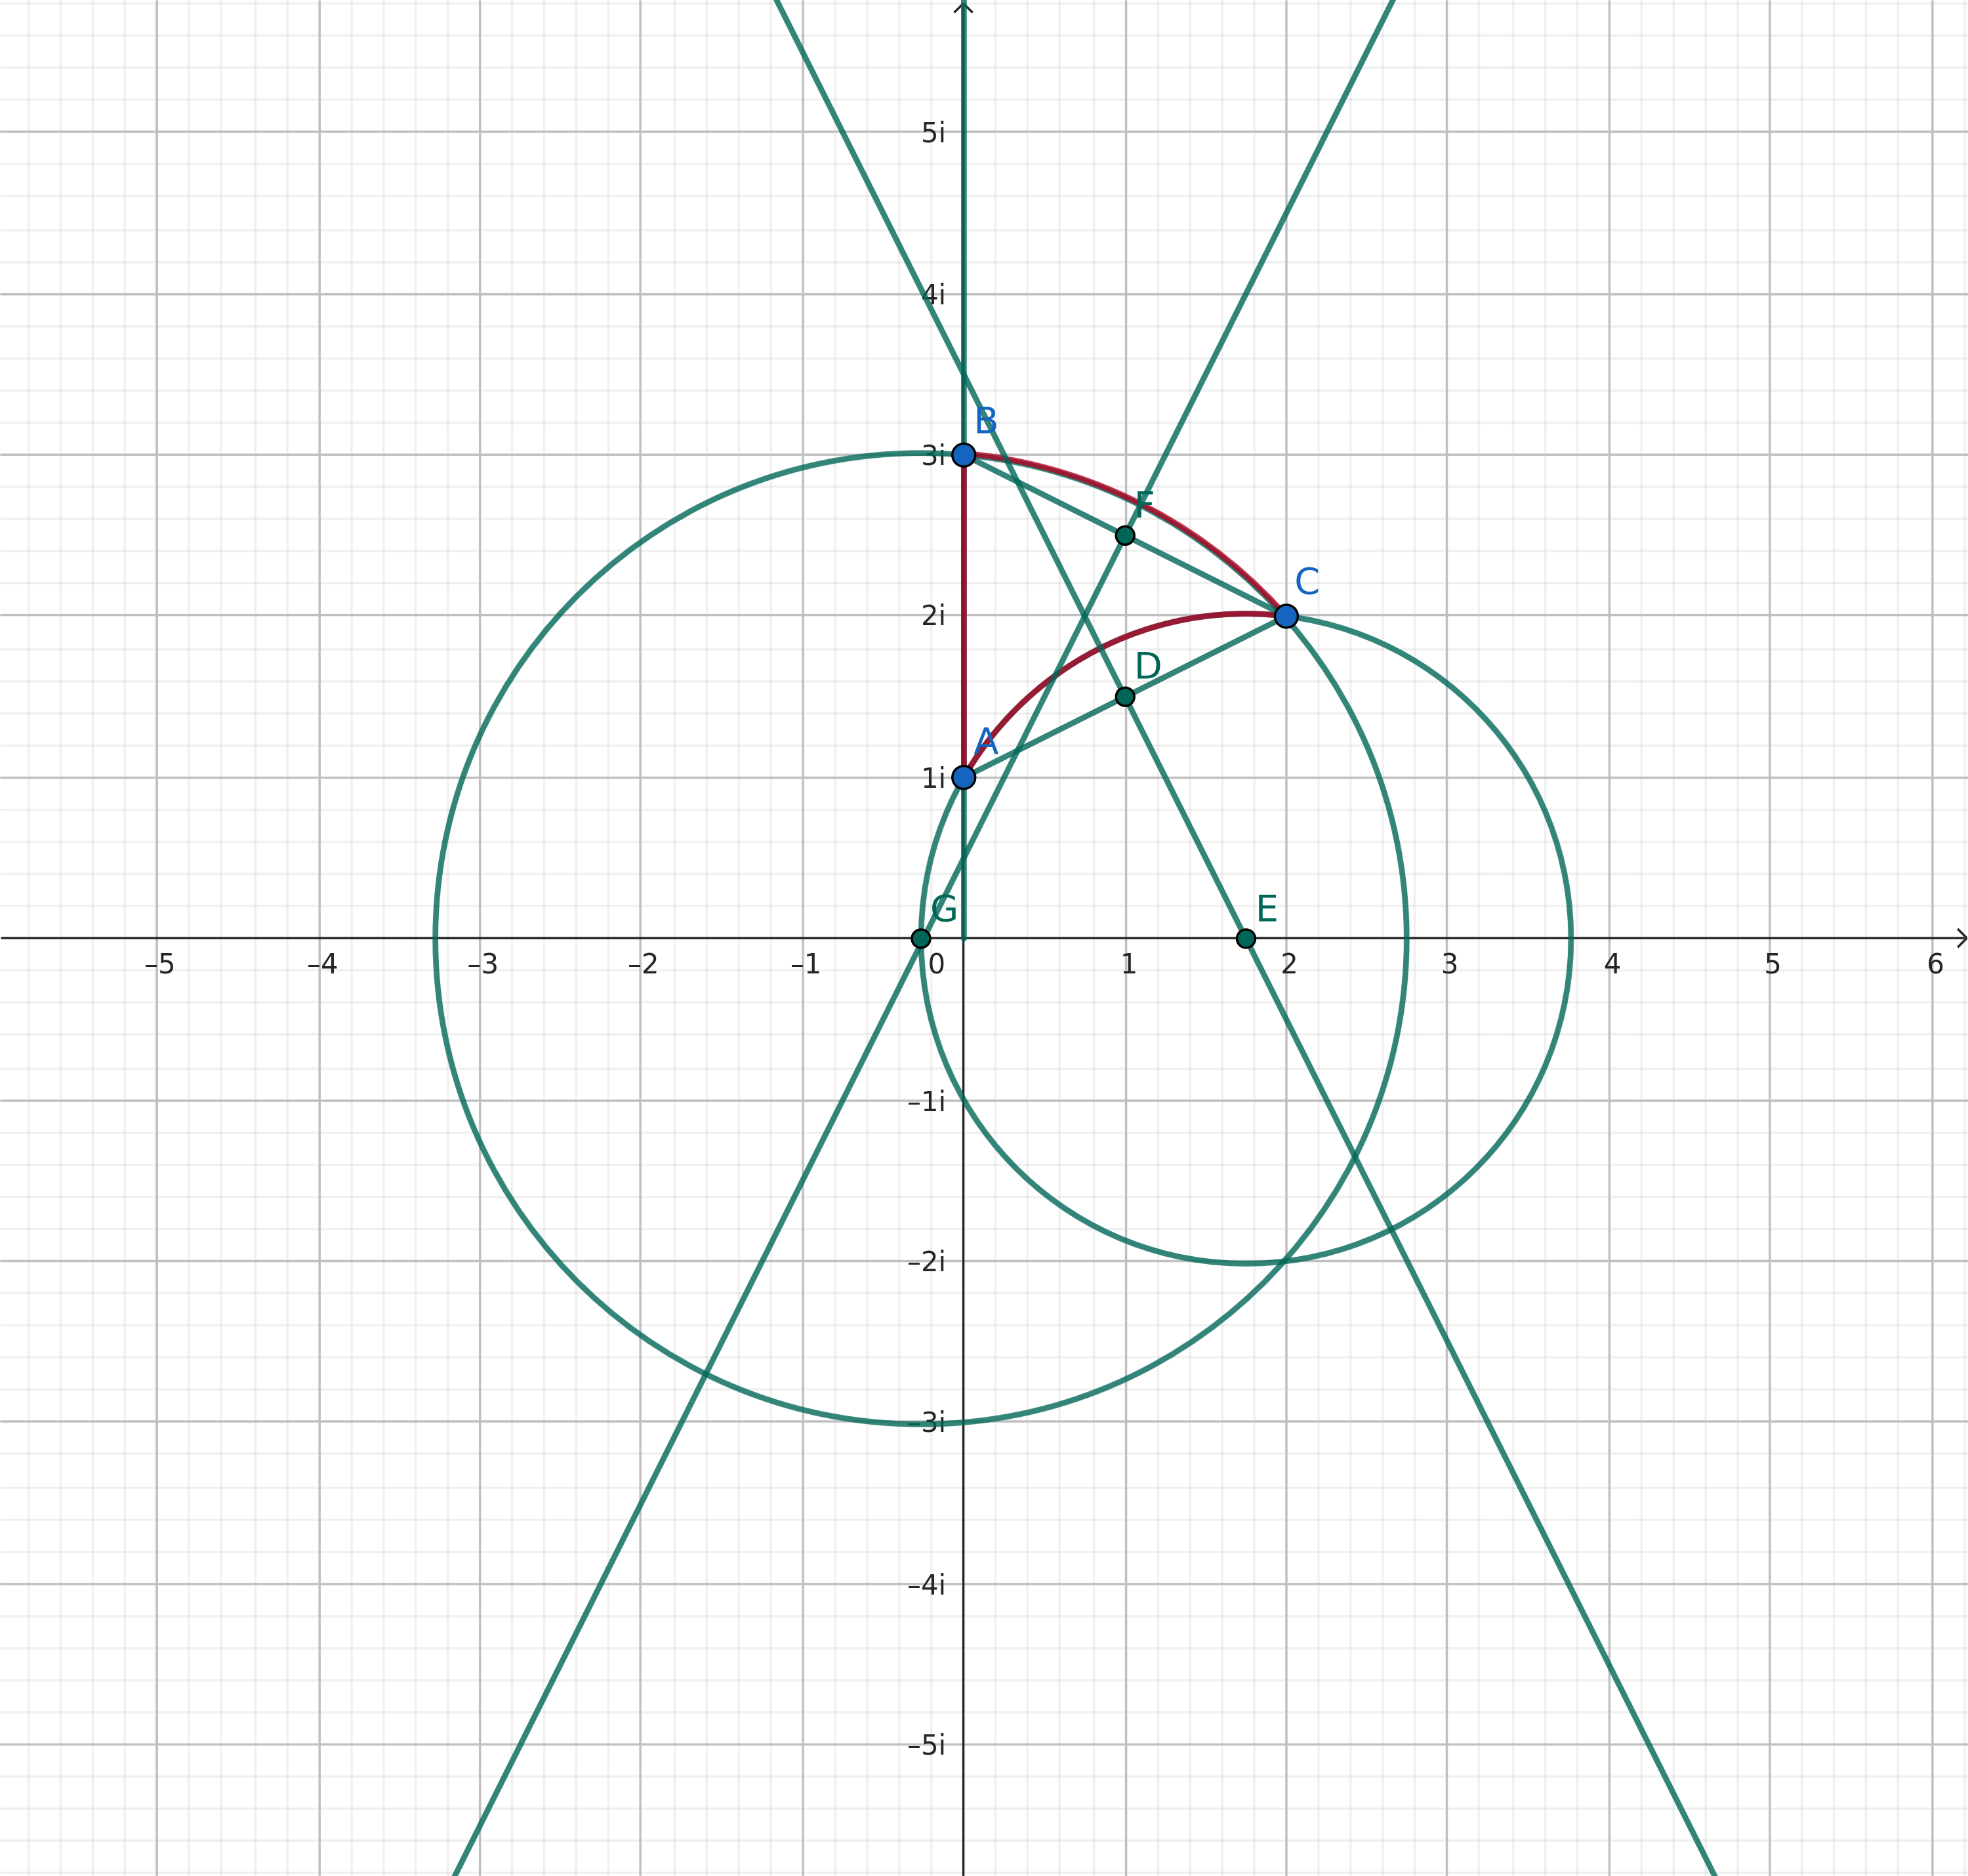
\includegraphics[width=0.8\textwidth]{Blatt07_Aufgabe_21}
    \caption{Hyperbolisches Dreieck}
    \label{fig:Aufgabe_21}
\end{figure}

\noindent Sei A der Punkt i, sei B der Punkt 3i und sei C der Punkt 2 + 2i. Zuerst verwendet man das Lineal und zeichnet den Strahl durch A und B ein (startet an der X-Achse). Dann konstruiert man die Mittelsenkrechte von B und C und bestimmt deren Schnittpunkt mit der X-Achse. Mit dem Zirkel am Schnittpunkt einstechen und einen Halbkreis durch B und C zeichnen. Analog den Halbkreis durch A und C einzeichnen. (Wie kann man eigentlich in Geogebra mit wenig Aufwand einen Halbkreis zeichnen? Man kann einen Kreisbogen zeichnen, dann muss man aber zuerst die Schnittpunkte mit der X-Achse bestimmen)

\subsection*{(iia)}
Sei P = ai und Q = bi für b>a>0.\\
Dann ist 
\begin{align*}
    d_{\mathbb{H}}(P, Q) &= arcosh \left( 1 + \frac{|Q - P|^{2}}{2Im(P)Im(Q)} \right) =arcosh \left( 1 + \frac{|(b-a)i|^{2}}{2Im(P)Im(Q)} \right) \\
                         &= arcosh \left( 1 + \frac{\sqrt{(b - a)^2}^{2}}{2ba} \right) = arcosh \left( 1 + \frac{(b - a)^{2}}{2ba} \right) \\
                         &= arcosh \left( 1 + \frac{b^2 - 2ba + a^2}{2ba} \right) = arcosh \left( 1 + \frac{2ba \cdot (\frac{b}{2a} - 1 + \frac{a}{2b}}{2ba} \right) \\
                         &= arcosh \left( \frac{b^2 + a^2}{2ba} \right) = arcosh \left( \frac{a^2 \cdot (\frac{b^2}{a^2} + 1)}{a^2 \cdot 2 \frac{b}{a}} \right) = arcosh \left( \frac{\left(\frac{b}{a}\right)^2 + 1}{2 \frac{b}{a}} \right) \\ 
                         &= ln\left( \frac{b}{a} \right)
\end{align*}

\subsection*{(iib)}
Sei M = ci der Mittelpunkt von $\overline{PQ}$. Dann ist: \\
\begin{align*}
ln\left(\frac{b}{c}\right) = ln\left(\frac{c}{a}\right) \Leftrightarrow \frac{b}{c} = \frac{c}{a} \Leftrightarrow c^2 = ab
\end{align*}

\subsection*{(iic)}
\end{document}
